% !TEX root = ../main.tex

\chapter{Conclusione e Lavori Futuri}\label{chap9:Concl}
Questa tesi ha proposto una metodologia al fine di verificare l'esistenza di una nuova classe ipotizzata in altri lavori, chiamata preFoG, che si pone come fase di transizione tra un attività normale ed un episodio di Freezing. Riconoscere questa nuova classe permette lo sviluppo di una procedura di previsione del FoG, al fine di far verificare meno episodi possibili di Freezing. Un primo studio dei dati attraverso l'uso di un discriminante lineare ci ha permesso di mostrare e quindi verificare l'effettiva esistenza di questa classe, anche se con una certa sovrapposizione con le altre classi già presenti, dato che al suo interno può contenere movimenti simili a quelli presenti nelle altre classi.\\ 
Per trovare la migliore divisione tra le varie classi, é stato condotto uno studio sulle tempistiche temporali, in cui si é cercato di capire quale fosse la migliore scelta di durata della finestra di divisione dei dati e con quale sovrapposizione. Lo studio é stato condotto sia tramite LDA che con degli approcci di clustering. Questi sono stati usati in quanto permettono un apprendimento non supervisionato dei dati, e quindi l'uso di tali procedimenti potrebbe sostituire il lavoro di etichettatura del dottore stesso. Tale studio ci ha portati a definire una finestra di 2 secondi con overlap di 1 secondo come durata migliore degli intervalli temporali al fine di dividere le varie classi. Per la fase non supervisionata di etichettatura dei dati al fine di sostituire il dottore, si é arrivati ad un'accuratezza massima del 91\%, con una media, tra i vari pazienti, intorno al 75\%, anche se si hanno ancora dei valori non ottimali per quanto riguarda precisione e recall. Per quei pazienti che non hanno presentato episodi di FoG, comunque, gli algoritmi sono riusciti ad evidenziare tale fatto, il che ci porta a rinforzare l'idea che i movimenti di camminata normale siano differenti sia da quelli di preFoG che di FoG.\\
L'intervallo migliore poi é stato usato per sviluppare un approccio di classificazione tramite LDA, al fine di etichettare nuovi dati. Questo é stato applicato sia su singoli pazienti che su tutti i dati di un test del dataset, al fine di verificare se i movimenti del preFoG fossero simili tra i vari pazienti. Per fare questo, sono state unite le classi di noFOG e FoG, mentre é stata tenuta separata quella di preFoG. Attraverso un processo di cross-validation sui singoli pazienti, questo ci ha portato ad un'accuratezza del 100\%, quindi un riconoscimento perfetto delle occorrenze all'interno dello stesso percorso del paziente. Sui dati di tutti i pazienti, invece, la cross-validation ci ha portati ad un'accuratezza del 90\% e valori simili anche per quanto riguarda la sensitività, specificità e F1-measure, dando ulteriore conferma che i movimenti di preFoG sono più o meno simili anche tra pazienti diversi, almeno all'interno di uno stesso percorso. Questo risultato migliora quanto fatto in \cite{12}, dove attraverso lo stesso test raggiungevano una misura di F1-measure del 75\%.\\
Per quanto riguarda la predizione su nuovi dati, invece, c'é sicuramente ancora lavoro da fare, in quanto i primi test ci hanno portato ad un'alta sensitività ma ad una bassa specificità, il che vuol dire che il classificatore tende a confondere i preFoG quando al paziente si danno da seguire percorsi differenti.
\section{Lavori Futuri}
Tra i possibili lavori futuri c'é sicuramente da continuare sulla classificazione di nuovi dati, andando a migliore quanto più possibile specialmente la specificità della previsione. Questo potrebbe essere svolto anche analizzando algoritmi di classificazione differenti dal knn, magari più complessi ed in grado di catturare in maniera migliore le similarità e le divisioni tra le varie classi.\\
Un altro lavoro possibile é quello di cercare una diversa metodologia di estrazione delle feature per quanto riguarda la procedura di clustering e quindi il tentativo di sostituzione del dottore nella prima fase di test. Questo può essere fatto, per esempio, scegliendo nuove feature da calcolare.\\
Un ulteriore lavoro futuro, e sicuramente il più interessante ed utile, é quello di applicare tali algoritmi di classificazione e clustering in dispositivi indossabili nella vita quotidiana dal paziente. Questo permetterebbe un riconoscimento real-time delle occorrenze di preFoG per evitare i Freezing e quindi permettere al paziente di bloccarsi il meno possibile. Un ipotetico schema di lavoro é quello presentato in \ref{LavoroFuturo}.

\begin{figure}[]
	\centering
	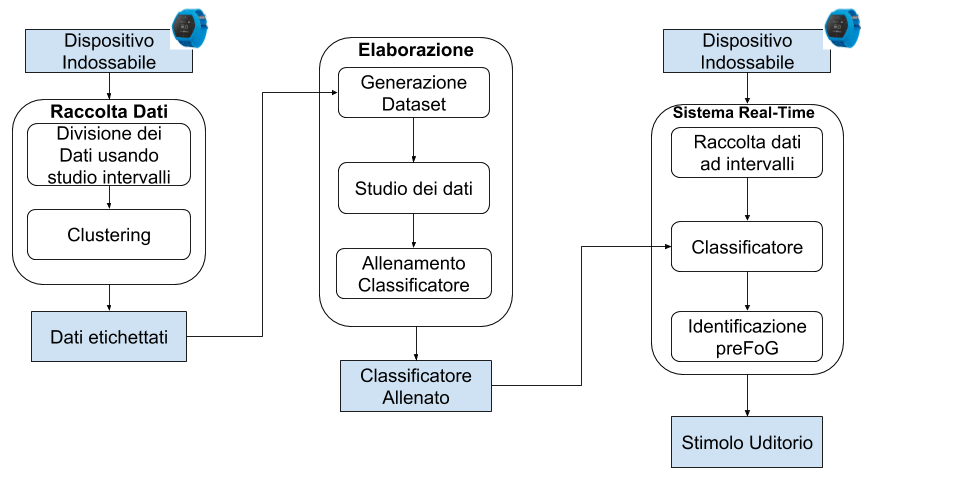
\includegraphics[scale=0.6,angle=90]{images/LavoroFuturo.png}
	\caption{Possibile schema di sistema real-time per l'identificazione del preFoG}
	\label{LavoroFuturo}
\end{figure}